\documentclass[a4paper,10pt]{article}


\usepackage{listings}

%Math
\usepackage{amsmath}
\usepackage{amsfonts}
\usepackage{amssymb}
\usepackage{amsthm}
\usepackage{ulem}
\usepackage{stmaryrd} %f\UTF{00FC}r Blitz!

%PageStyle
\usepackage[german]{babel}
\usepackage{fontenc}
\usepackage{fancyhdr, graphicx}
\usepackage{wasysym}
\usepackage{fullpage}
\usepackage{textcomp}
\usepackage{fancyhdr} %for header/footer

%My Commands
\newcommand{\BN}{\mathbb{B}} %BOOL
\newcommand{\RN}{\mathbb{R}} %Real Number
\newcommand{\NN}{\mathbb{N}} %Natural Number
\newcommand{\QN}{\mathbb{Q}} %Rational Number
\newcommand{\ZN}{\mathbb{Z}} %ganze Zahlen
\newcommand{\CN}{\mathbb{C}}
\newcommand{\Teilt}{\mid} %|
\newcommand{\Teiltn}{\nmid} %kein teiler
\newcommand{\Potp}{\mathcal{P}} %Potenzmenge
\newcommand{\Pota}{\mathcal{A}}
\newcommand{\Potr}{\mathcal{R}}
\newcommand{\Potn}{\mathcal{N}}
\newcommand{\Bold}[1]{\textbf{#1}} %Boldface
\newcommand{\Kursiv}[1]{\textit{#1}} %Italic
\newcommand{\T}[1]{\text{#1}} %Textmode
\newcommand{\Nicht}[1]{\T{\sout{$ #1 $}}} %Streicht Shit durch
\newcommand{\lra}{\leftrightarrow} %Arrows
\newcommand{\ra}{\rightarrow}
\newcommand{\la}{\leftarrow}
\newcommand{\lral}{\longleftrightarrow}
\newcommand{\ral}{\longrightarrow}
\newcommand{\lal}{\longleftarrow}
\newcommand{\Lra}{\Leftrightarrow}
\newcommand{\Ra}{\Rightarrow}
\newcommand{\La}{\Leftarrow}
\newcommand{\Lral}{\Longleftrightarrow}
\newcommand{\Ral}{\Longrightarrow}
\newcommand{\Lal}{\Longleftarrow}
\newcommand{\Vektor}[1]{\vec{#1}}
\newcommand{\Brace}[1]{\left( #1 \right)} %()
\newcommand{\Bracel}[1]{\left\lbrace #1 \right.} %(
\newcommand{\Bracer}[1]{\right. #1 \right\rbrace} %)
\newcommand{\Brack}[1]{\left\lbrace #1 \right\rbrace} %{}
\newcommand{\Brackl}[1]{\left\lbrace #1 \right.} %{
\newcommand{\Brackr}[1]{\right. #1 \right\rbrace} %}
\newcommand{\Result}[1]{\underline{\underline{#1}}} %Doppelt unterstrichen
\newcommand{\Abs}[1]{\left| #1 \right|} %Absolutbetrag
\newcommand{\Norm}[1]{\Abs{\Abs{ #1 }}} %Norm
\newcommand{\Arrays}[1]{\left(\begin{array}{c}#1\end{array}\right)} %Array mit einer Kolonne ()
\newcommand{\Array}[2]{\left(\begin{array}{#1}#2\end{array}\right)} %Array mit n Kolonnen ()
\newcommand{\Bracka}[2]{\left\lbrace\begin{array}{#1}#2\end{array}\right\rbrace} %Array mit {}
\newcommand{\Brackal}[2]{\left\lbrace\begin{array}{#1} #2 \end{array}\right.} %Array mit {
\newcommand{\Brackar}[2]{\left.\begin{array}{#1} #2 \end{array}\right\rbrace} %Array mit }
\newcommand{\Sumone}[2]{\sum_{#2=1}^{#1}} %Summe von 1
\newcommand{\Sumz}[2]{\sum_{#2=0}^{#1}} %Summe von 0
\newcommand{\Sum}[2]{\sum_{#2}^{#1}} %Allgemeine Summe
\newcommand{\Oneover}[1]{\frac{1}{#1}} %1 \UTF{00FC}ber igendwas
\newcommand{\Tablewt}[3]{\begin{table*}[h]\caption{#1} \begin{tabular}{#2}{#3}\end{tabular}\end{table*}} %Table mit Titel
\newcommand{\Oben}[2]{\overset{#1}{#2}} %etwas \UTF{00FC}ber etwas anderem
\newcommand{\Unten}[2]{\underset{#1}{#2}} %etwas unter etwas anderem
\newcommand{\Bildcap}[2]{\begin{figure}[htb]\centering\includegraphics[width=0.2\textwidth]{#1} \caption{#2}\end{figure}} %Bild mit beschriftung
\newcommand{\Bildjpeg}[1]{\includegraphics[width=0.2\textwidth]{#1.jpeg}} %Bilder jpeg!!
\newcommand{\Bildjpg}[1]{\includegraphics[width=0.2\textwidth]{#1.jpg}} %Bilder jpg!!

%Zeichnung
\usepackage{tikz}
\usepackage[all]{xy}
\usepackage{ucs}

\definecolor{dkgreen}{rgb}{0,0.6,0}
\definecolor{gray}{rgb}{0.5,0.5,0.5}
\definecolor{mauve}{rgb}{0.58,0,0.82}
 
\lstset{ %
  language=Octave,                % the language of the code
  basicstyle=\footnotesize,           % the size of the fonts that are used for the code
  numbers=left,                   % where to put the line-numbers
  numberstyle=\tiny\color{black},  % the style that is used for the line-numbers
  stepnumber=1,                   % the step between two line-numbers. If it's 1, each line 
                                  % will be numbered
  numbersep=5pt,                  % how far the line-numbers are from the code
  backgroundcolor=\color{white},      % choose the background color. You must add \usepackage{color}
  showspaces=false,               % show spaces adding particular underscores
  showstringspaces=false,         % underline spaces within strings
  showtabs=false,                 % show tabs within strings adding particular underscores
  tabsize=2,                      % sets default tabsize to 2 spaces
  captionpos=b,                   % sets the caption-position to bottom
  breaklines=true,                % sets automatic line breaking
  breakatwhitespace=false,        % sets if automatic breaks should only happen at whitespace
  keywordstyle=\color{blue},          % keyword style
  commentstyle=\color{black},       % comment style
  stringstyle=\color{mauve},         % string literal style
  morekeywords={int,long,float,public,static,class}               % if you want to add more keywords to the set
}

%Config
\renewcommand{\headrulewidth}{0pt}
\setlength{\headheight}{15.2pt}
\pagestyle{plain}

%Metadata
\title{Algorithmen und Datenstrukturen}
\author{Jan F\"assler}
\date{2. Semester (FS 2012)}
\fancyfoot[C]{Jan F\"assler}

\begin{document}
\maketitle
\newpage
\thispagestyle{fancy} %f\UTF{00FC}r Header

\section{Daten \& Informationenen}

\subsection{Digitaltechnik}
\begin{tabular}{l l l}
	0 & low & 0 bis 0.8V \\
	1 & high & 2.4 bis 5V
\end{tabular} \\ \\
Mit einer Bitfolge der L\"ange n k\"onnen $2^n$ verschiedene Zust\"ande codiert werden.

\subsection{Byte}
\begin{itemize}
	\item geordnete Bitfolge der L\"ange 8 (256 Zust\"ande)
	\item Bits werden mit Indizes von 0 bis 7 nummeriert
	\item LSB (Least Significant Bit)
	\item MSB (Most Significant Bit)
\end{itemize}
\begin{tabular}{l l}
	KiByte & $2^{10}$ Byte \\
	MiByte & $2^{20}$ Byte \\
	GiByte & $2^{30}$ Byte \\
\end{tabular}

\subsection{Zahlendarstellung}
\begin{description}
	\item[bin\"ar (2)] - Zahlen die mit 0b beginnen
	\item[octal (8)] - Zahlen die mit 0 beginnen
	\item[dezimal (10)] - Zahlen die nicht mit 0 beginnen
	\item[hex (16)] - Zahlen die mit 0x beginnen
\end{description}
Positive Zahlen: $\sum b_i+B^i$ mit $i \in [0,n-1]$ und $b_i$ gleich der Ziffer bei $i$. \\ \\
Ganze Zahlen: $-b_{n-1}*B^{n-1}+\sum b_i*B^i$ mit $i \in [0,n-2]$ und  $b_i$ Ziffer bei $i$.

\subsection{Datentypen in JAVA}
\begin{tabular}{l c c l l}
	Name & Byte & Bit & kleinste Zahl & gr\"osste Zahl \\
	\hline
	\Bold {byte} & 1 & 8 & -127 & 128 \\
	\Bold {short} & 2 & 16 &-32.768 & 32.767 \\
	\Bold {char} & 2 & 16 & $\backslash$u0000 (0) & 	$\backslash$uFFFF (65.535) \\
	\Bold {int} & 4 & 32 & -2.147.483.648 & 2.147.483.647 \\
	\Bold {long} & 8 & 64 & -9.223.372.036.854.775.808 & 9.223.372.036.854.775.807 \\
	\Bold {float} & 4 & 32 & $1,40 * 10^{-45}$ & $3,40282346638528860 * 10^{38}$ \\
	\Bold {double} & 8 & 64 & $4,94065645841246544*10^{-324}$ & $1,79769313486231570*10^{308}$  \\
\end{tabular}

\subsection{Ganze Zahlen}

\subsubsection{Positive Zahlen}
\begin{tabular}{c c c c c c c c}
	1 & 0 & 1 & 0 & 0 & 1 & 1 & 1 \\
	$2^7$ & $2^6$ & $2^5$ & $2^4$ & $2^3$ & $2^2$ & $2^1$ & $2^0$
\end{tabular}
$1*2^7+1*2^5+1*2^2+1*2^1+1*2^0=128+32+4+2+1=\uuline{167}$

\subsubsection{Negative Zahlen (2er - Komplement)}
\begin{tabular}{c c c c c c c c}
	1 & 0 & 1 & 0 & 0 & 1 & 1 & 1 \\
	$2^7$ & $2^6$ & $2^5$ & $2^4$ & $2^3$ & $2^2$ & $2^1$ & $2^0$
\end{tabular} 
$-1*2^7+1*2^5+1*2^2+1*2^1+1*2^0=-128+32+4+2+1=\uuline{-89}$



\subsection{Gleitkommazahlen}
Exponentialdarstellung: $(-1)^V * (1+M)*2^E$ \\
IEEE 754 Float: $(-1)^V * (1+M) * 2^{E-127}$ \\
IEEE 754 Double: $(-1)^V * (1+M) * 2^{E-1023}$ \\
\begin{description}
	\item[V] - Vorzeichen (float 1Bit / double 1 Bit)
	\item[M] - normalisierte Mantrisse $(0 \leq M \leq 1)$ (float: 23 Bits / double: 52 Bits)
	\item[E] - Exponent (float: Signed-8-Bit $-$ 127  / double: Signed-11-Bit $-$ 1023)
\end{description} 
\begin{tabular}{|c|l|l|}
	\hline
	V & Exponent & Mantrisse \\
	\hline
\end{tabular}

\subsubsection{Beispiele (IEEE 754 32bit Float)}
\begin{description}
	\item[2.5] $=1.25*2^1$
	\item[-0.75] $=\underbrace{1}_{\ominus}\underbrace{01111110}_{126 - 127} \underbrace{100000...}_{1+2^{-1}}=-1.5*2^{-1}$
	\item[0.1] $=\underbrace{0}_{\oplus}\underbrace{01111011}_{123 - 127} \underbrace{100\overline{1100}.........}_{1+2^{-1}+2^{-4}+2^{-5}...}=1.6*2^{-4} = 0.100000001490116119384765625$ 
	\item Umrechnen von $-1313.3125$ zu IEEE 32-bit float:
	\begin{enumerate}
		\item Ganzzahlteil $1313_{10}=10100100001_2.$
		\item Nachkommateil\\
		\begin{tabular}{lll}
			0.3125&$\times2=0.625$& \Bold{0}\\
			0.625&$\times 2=1.25$ &\Bold{1}\\
			0.25&$\times 2 = 0.5$ &\Bold{0}\\
			0.5&$\times 2=1.0$ &\Bold{1}\\
		\end{tabular}
		\item $1313.3125_{10}=10100100001.0101_2$
		\item Normen $10100100001.0101_2=1.01001000010101_2\times2^{10}$
		\item Mantisse ist $01001000010101$, Exponent ist $10 + 127 = 137 = 10001001_2$, Vorzeichen ist 1.
		\item -1313.3125 ist 
		\begin{tabular}{|c|l|l|}
		\hline
		1 & 10001001 & 01001000010101000000000 \\
		\hline
	\end{tabular}
	\end{enumerate} 
\end{description}

\subsubsection{Spezialf\"alle}
\begin{description}
	\item[E=00000000 M=0] $\Rightarrow 0$
	\item[E=11111111 M=0 V=+] $\Rightarrow +\infty$
	\item[E=11111111 M=0 V=$-$] $\Rightarrow -\infty$
	\item[E=11111111 M$\neq$0] $\Rightarrow NaN$
\end{description}

\subsubsection{Division mit Null}
\begin{itemize}
	\item float f = $\pm$0.0f/$\pm$0.0f = $NaN$
	\item float f = 7.6f/0.0f = -7.6f/-0.0f = $+\infty$
	\item float f = -3.9f/0.0f = 3.9f/-0.0f = $-\infty$
\end{itemize}

\newpage
\section{Operationen \& Ausdr\"ucke}

\subsection{Auswertungsreihenfolge}
\begin{itemize}
	\item einstellige und mehrstellige Operatoren
		\begin{itemize}
			\item[1.] Teilausdr\"ucke in Klammern
			\item[2.] Ausdr\"ucke mit un\"aren Operatoren (pro Operand von rechts nach links)
			\item[3.] Teilausdr\"ucke mit mehrstelligen Operatoren gem\"ass Priorit\"atstabelle
		\end{itemize}
	\item mehrstellige Operatoren gleicher Priorit\"at \\
		bei gleicher Priorit\"at entscheidet die Assoziativit\"at (von links nach rechts oder von rechts nach links)
	\item Bewertungsreihenfolge von Operanden \\
		die Operanden eines Operators werden strikt von links nach rechts ausgewertet
\end{itemize}
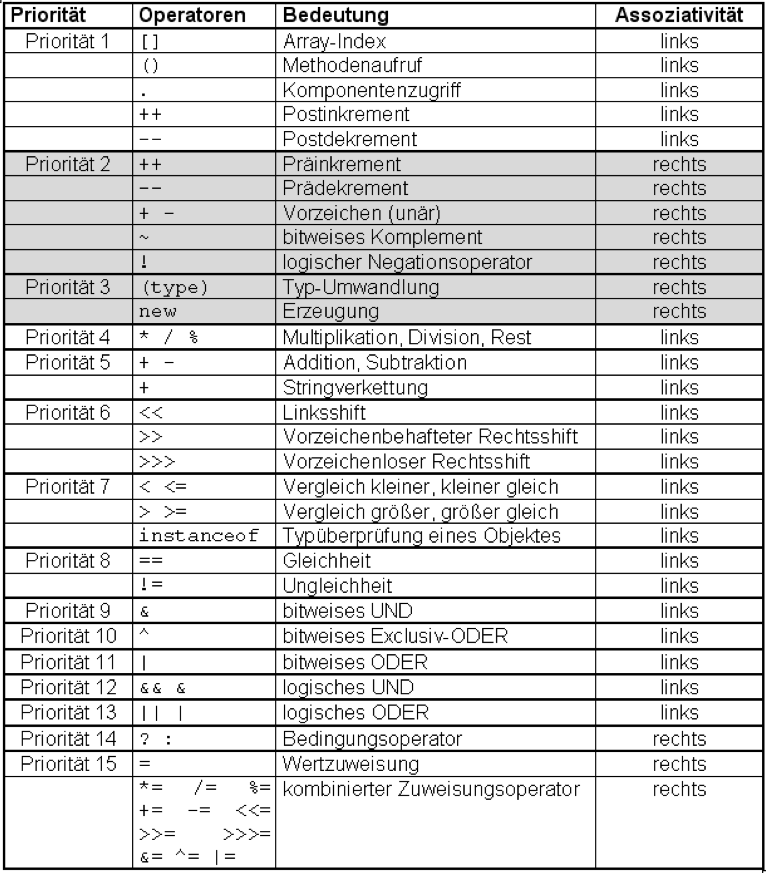
\includegraphics[width=150mm]{operatoren_prios.png}

\subsection{Bitoperatoren}
logische oder auch boolesche Operatoren: \\
\begin{tabular}{|c|c|c|c|c|c|}
	\hline
	& & \Bold {AND} & \Bold {OR} & \Bold {Negation} & \Bold {XOR} \\
	\Bold {a} & \Bold {b} & \Bold {a \& b} & \Bold {a $|$ b} & \Bold {$\sim$a} & \Bold {a $\wedge$  b} \\
	\hline
	0 & 0 & 0 & 0 & 1 & 0 \\
	0 & 1 & 0 & 1 & 1 & 1 \\
	1 & 0 & 0 & 1 & 0 & 1 \\
	1 & 1 & 1 & 1 & 0 & 0 \\
	\hline
\end{tabular}

\subsection{Schiebeoperatoren}
\begin{itemize}
	\item \Bold {Rechtsschiebe-Operatoren}
		\begin{itemize}
			\item vorzeichenbehaftet: $a >> b$, \Bold{Bsp:}$-9_{10} = 11110111_2 >> 1 = 11111011_2 = -5_{10}$
			\item vorzeichenlos: $a >>> b$, \Bold{Bsp:}$-9_{10} =  11110111_2 >>> 1 = 01111011_2 = 123_{10}$ 
		\end{itemize}
	\item \Bold {Linksschiebe-Operator}
		\begin{itemize}
			\item kann Vorzeichen ver\"andern:  $a << b$
		\end{itemize}
\end{itemize}

\subsection{Logische Operatoren}
\begin{description}
	\item[logische Negation:] !A
	\item[logisches UND:] A \&\& B  / A \& B \\
				(Bei zwei \& Zeichen wird erst A \"uberpr\"uft und B nur, falls A wahr ist.)
	\item[logisches ODER:] A $||$ B / A $|$ B
	\item[Bedingungsoperator:] A ? B : C (if (A) then B else C)
\end{description}

\subsection{Konvertierung von Datentypen}

\subsubsection{explizite Typkonvertierung}
\begin{itemize}
	\item Konvertierungen sind m\"oglich:
		\begin{itemize}
			\item zwischen numerischen Datentypen (\Bold {erweiternd und einschr\"ankend})
			\item zwischen Referenztypen
		\end{itemize}
	\item funktionieren gleich wie implizite, allerdings bestehen mehr M\"oglichkeiten
	\item cast-Operator: (Typname) Ausdruck
\end{itemize}

\subsubsection{implizite (automatische) Typkonvertierung}
\begin{itemize}
	\item zwischen Operanden von numerischem Typ (\Bold {nur erweiternd})
	\item zwischen Operanden von Referenztypen
	\item bei Verkn\"upfungen von String-Objekten mit Operanden anderer Typen \\
			    Object o = new Object();\\
			    String s = $"$X$"$+null+o;\\
			   String s = $"$X$"$+$"$null$"$+o.toString();\\
                                   String s = $"$Xnulljava.lang.Object@47ac1adf$"$;
	\item arithmetische Operatoren: Konvertierung in h\"oheren Typ gem\"ass Hierarchie
\end{itemize}

\subsubsection{erweiternde Typkonvertierungen}
		Wert ist immer darstellbar \\
		m\"oglicher Verlust an Genauigkeit (z.B. bei Konvertierung von int nach float) \\ \\
		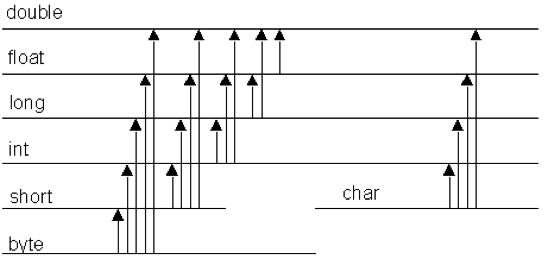
\includegraphics[width=75mm]{erweiternde_typumwandlung.png} \\
		
\subsubsection{einschr\"ankende Typkonvertierungen}
		m\"oglicher Informationsverlust in Gr\"osse, Vorzeichen \& Genauigkeit \\ \\
		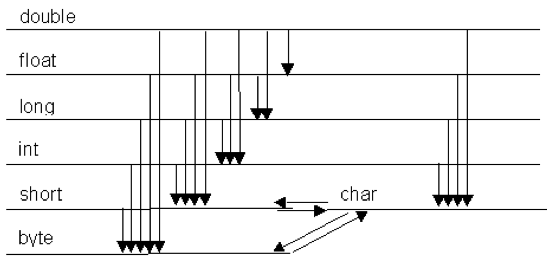
\includegraphics[width=75mm]{einschraenkende_typumwandlung.png}


\subsubsection{Integer-Erweiterung}
\begin{itemize}
	\item Datentypen byte, short und char werden in Ausdr\"ucken mit un\"aren und bin\"aren Operatoren implizit in int konvertiert
		\begin{itemize}
			\item Dimensionsausdruck bei der Erzeugung von Arrays
			\item Indexausdruck in Arrays
			\item Operand der un\"aren Operatoren $+$ und $ - $
			\item Operand des Invertierungsoperators f\"ur Bits $\sim$
			\item Operanden der Schiebeoperatoren $>>$, $>>>$ und $<<$
		\end{itemize}
	\item byte, short und char werden somit fast ausschliesslich als Datenfelder f\"ur Klassen benutzt
\end{itemize}

\subsubsection{Konvertierungsvorschriften}
\begin{itemize}
	\item erweiternde Konvertierung von vorzeichenbehafteten Integer-Typen \\
		Wert bleibt unver\"andert
	\item Konvertierung zwischen char und vorzeichenbehafteten Integer-Typen
		\begin{itemize}
			\item char ist vorzeichenlos
			\item bei gleicher Breite: Bitmuster bleibt erhalten
			\item char ist breiter: von links mit Nullen auff\"ullen und Vorzeichen propagieren
			\item char ist schmaler: kein korrektes Resultat, wenn Wert gr\"osser als $2^{16}$
		\end{itemize}
	\item Konvertierung von Integer nach Gleitpunkt \\
		n\"achst h\"oherer oder niedriger darstellbarer Wert
	\item Konvertierung von Gleitpunkt nach Integer
		\begin{itemize}
			\item Nachkommastellen werden abgeschnitten
			\item bei Werten gr\"osser als $2^{31} - 1$ ist das Resultat nicht korrekt ($= 2^{31} - 1$)
		\end{itemize}
	\item Konvertierung zwischen Gleitpunkt-Typen
		\begin{itemize}
			\item float nach double: Wert bleibt unver\"andert
			\item double nach float: Wert im zul\"assigen Wertebereich von float, dann n\"achst h\"oherer oder niedriger darstellbarer Wert
		\end{itemize}
\end{itemize}

\subsection{Code-Listings}

\subsubsection{1er-Bits z\"ahlen}
\begin{lstlisting}
public static int count(int x) {
	final int intSize = 32;  // Anzahl Bits einer Integer-Zahl
	int y = 0;               // output
	for (int i=0; i < intSize; i++) { 
		if (x%2 == 1) y++;
		x >>>= 1;
	}
	return y;
}

\end{lstlisting}

\subsubsection{effizienter Z\"ahler der 1er-Bits}
\begin{lstlisting}
public static int countEfficiently(int x) {
	int iEven, iOdd, d = 1;
	iEven = x & 0x55555555; x >>= d; iOdd = x & 0x55555555; 
	x = iOdd + iEven; d <<= 1 ;
	iEven = x & 0x33333333; x >>= d; iOdd = x & 0x33333333; 
	x = iOdd + iEven; d <<= 1 ;	
	iEven = x & 0x0F0F0F0F; x >>= d; iOdd = x & 0x0F0F0F0F; 
	x = iOdd + iEven; d <<= 1;	
	iEven = x & 0x00FF00FF; x >>= d; iOdd = x & 0x00FF00FF; 
	x = iOdd + iEven; d <<= 1 ;
	iEven = x & 0x0000FFFF; x >>= d; iOdd = x & 0x0000FFFF; 
	x = iOdd + iEven; d <<= 1 ;	
	return x;
}
\end{lstlisting}

\subsubsection{Ganzzahlige Addition}
\begin{lstlisting}
public static int add(int a, int b) {
	int c, r, t; // output r = a + b
	r = a^b; // Addition entspricht fast einer XOR-Operation 
	c = a&b; // Carry-Flags bestimmen
	while (c != 0) { // Carry-Flags hinzuaddieren
		c <<= 1;
		t = r; r ^= c; c &= t;
	}
	return r;
}
\end{lstlisting}

\subsubsection{Ganzzahlige Multiplikation}
\begin{lstlisting}
public static long mult(int a, int b) {
	long y = 0; // output y = a*b
	while (a != 0) {
		if (a%2 == 1) y += b; 
		b <<= 1;
		a >>= 1;
	}
	return y;
}
\end{lstlisting}

\newpage
\section{Zeichen und Strings}
\subsection{Standardisierte Zeichencodierungen}
\subsubsection{ASCII (American Standard Code for Information Interchange)}
\begin{itemize}
	\item nur 128 verschiedene Zeichen (Steuerzeichen, Satzzeichen, Ziffern, Buchstaben usw.)
	\item pro Zeichen ein eindeutiger 7-Bit-Zeichencode
\end{itemize}
\subsubsection{ISO 8859-1 (Latin-1)}
\begin{itemize}
	\item 256 Zeichen f\"ur europ\"aische Sprachen (8-Bit-Zeichencode)
	\item die ersten 128 Zeichen sind identisch zu ASCII
	\item die zweiten 128 Zeichen enthalten europ\"aische Sonderzeichen, z.B. Umlaute
\end{itemize}
\subsubsection{Unicode}
\begin{itemize}
	\item \"uber eine Million Zeichen, verschiedene Sprachen (Arabisch, Hebr\"aisch, Chinesisch usw.)
	\item 21-Bit-Zeichencode: ersten 256 Zeichen sind identisch zu ISO 8859-1
\end{itemize}

\subsection{Java}
\subsubsection{Unicode in JAVA}
\begin{description}
	\item[Datentyp int] \hfill 
		\begin{itemize}
			\item 32-Bit im UTF-32 Format: nur die unteren 21 Bits werden benutzt, die oberen sind alle 0
			\item eine int-Variable kann jeden m\"oglichen Zeichencode (code point) des Unicodes aufnehmen
		\end{itemize}
	\item[Datentyp char] \hfill 
		\begin{itemize}
			\item 16-Bit (Codierungseinheit, code unit)
			\item eine char-Variable kann nur einen der ersten $2^{16}$ Zeichencodes des Unicodes (Basic Multilingual Plane, BMP) aufnehmen
			\item alle anderen Zeichencodes werden durch char-Paare codiert
		\end{itemize}
	\item[Interface CharSequence] \hfill 
		\begin{itemize}
			\item Sequenz von Zeichencodes im UTF-16 Format
			\item bekannte Implementierungen: String, StringBuffer, StringBuilder
		\end{itemize}
\end{description}

\subsubsection{Zeichenketten (Strings)}
\begin{description}
	\item[Character-Array] \hfill \\
		ver\"anderbare Zeichenkette mit expliziter L\"angenangabe (Teil des Arrays)
	\item[Klasse String (UTF-16 Format)] \hfill \\
		unver\"anderbare Zeichenkette mit expliziter L\"angenangabe
	\item[Klassen StringBuilder und StringBuffer (UTF-16 Format)] \hfill \\
		ver\"anderbare Zeichenkette gekapselt als abstrakter Datentyp
\end{description}

\subsubsection{String Funktionen}
\begin{description}
	\item[String equals(String vergleichenMit)] \hfill \\
		vergleicht den Inhalt von zwei Strings
	\item[String substring(int anfang, int ende)] \hfill \\
		Schneidet eine Zeichenkette zwischen Anfang und Ende –1 aus und erzeugt damit ein neues Stringobjekt. Der urspr\"ungliche String wird dabei nicht ver\"andert.
	\item[String trim()] \hfill \\
		Erzeugt Kopie und entfernt alle Leerzeichen am Anfang und Ende der Kopie. Die Kopie wird zur\"uckgegeben.
\end{description}

\subsection{Universal Character Encoding Standard (Unicode)}
\subsubsection{Coderaum}
\begin{description}
	\item[Ebene 0: Basic Multilingual Plane (BMP)] \hfill
		\begin{itemize}
			\item U+0 bis U+FFFF
			\item enth\"alt die wichtigsten Zeichen von verschiedenen Sprachen
		\end{itemize}
	\item[Ebene 1: Supplementary Multilingual Plane (SMP)] \hfill
		\begin{itemize}
			\item U+1'0000 bis U+1'FFFF
			\item enth\"alt weniger oft gebrauchte Zeichen (z.B. gotische Zeichen, Musiksymbole)
		\end{itemize}
	\item[Ebene 2: Supplementary Ideographic Plane (SIP)] \hfill
		\begin{itemize}
			\item U+2'0000 bis U+2'FFFF
			\item enth\"alt sehr seltene CJK Zeichen
		\end{itemize}
	\item[Ebene 3 bis 13] \hfill \\
		reserviert f\"ur sp\"atere Erg\"anzungen
	\item[Ebene 14: Supplementary Special-purpose Plane (SSP)] \hfill
		\begin{itemize}
			\item U+E'0000 bis U+E'FFFF
			\item enth\"alt zus\"atzliche Formatierungszeichen
		\end{itemize}
	\item[Ebenen 15 und 16: Private Use Planes] \hfill
		\begin{itemize}
			\item U+F'0000 bis U+F'FFFF und U+10'0000 bis 10'FFFF
			\item f\"ur private, nicht standardisierte Zwecke einsetzbar
		\end{itemize}
\end{description}

\subsubsection{UTF-32}
Dies ist die einfachste Umsetzung, es werden 21 Bits in einem (vorzeichenlosen) 32-Bit-Integer abgespeichert. Dabei sind die h\"oherwertigen 11 Bits immer null. Dies bedeutet jedoch eine grosse Speicherverschwendung

\subsubsection{UTF-16}
Dies ist ein guter Kompromiss zwischen Speicherbedarf und einfacher Handhabung. In diesem Standard werden Zeichencodes der BMP werden durch eine einzelne 16-Bit Codierungseinheit gespeichert. Die Zeichencodes der zus\"atzlichen Ebenen werden durch zwei 16-Bit Codierungseinheiten (Ersatzpaare) gespeichert. \\
Die beiden Zeichen eines Ersatzpaares stammen aus der Surrogates Area im BMP. Das erste Zeichen jeweils aus dem Bereich \Bold {U+D800 bis U+DBFF}. Das zweite Zeichen jeweils aus dem Bereich \Bold {U+DC00 bis U+DFFF}. Das ergiebt 2 mal 10 Bit Nutzdaten.

\subsubsection{UTF-8}
Dies ist ein sehr verbreiteter Standard in XML oder im Web. Er ist sehr speichereffizient f\"ur h\"aufige Zeichen und kompatibel mit dem ASCII Standard. F\"ur seltenere Zeichen ist er jedoch speicherineffizient und ist kompliziert in der Handhabung, da er aus 1 bis 4 Bytes besteht: \\
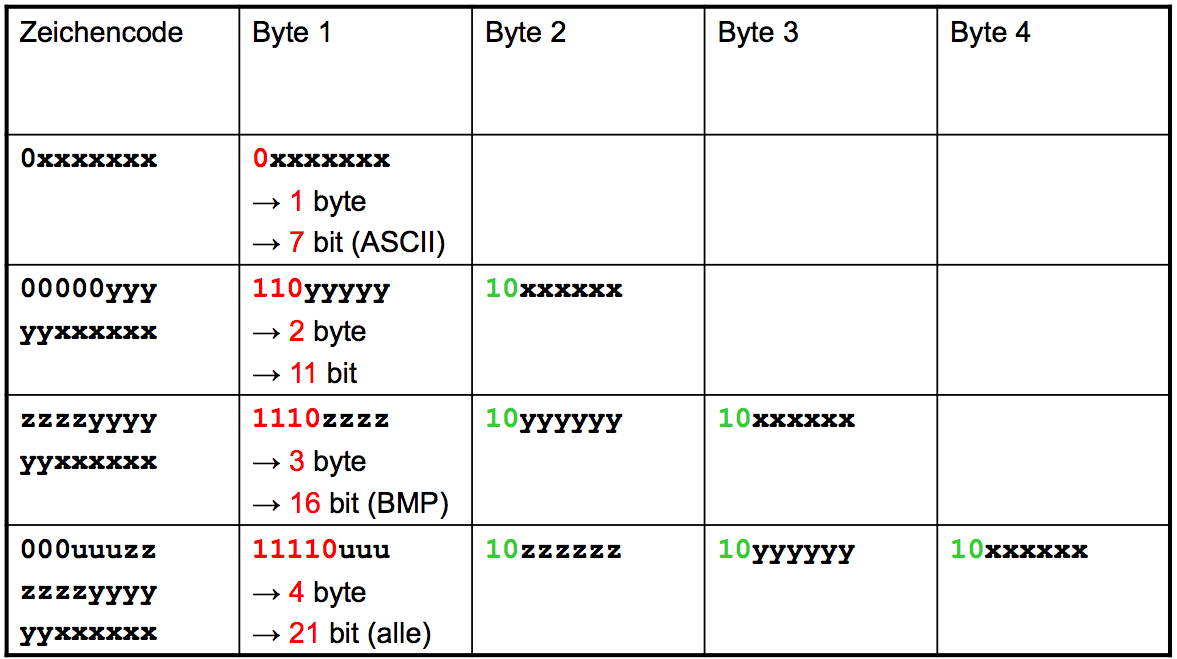
\includegraphics[scale=0.35]{utf8.png}

\subsubsection{Codierungsschemen}
Das bestimmt Codierungsformat und Byte-Reihenfolge:
\begin{itemize}
	\item bei Dateneinheiten bestehend aus mehreren Bytes muss festgehalten werden, welches Byte zuerst behandelt wird, das
		\begin{itemize}
			\item most significant byte (MSB) zuerst: big-endian
			\item least significant byte (LSB) zuerst: little-endian
 		\end{itemize}		 
 	\item relevant bei UTF-16 und UTF-32
 	\item nicht relevant bei UTF-8 (die Reihenfolge ist klar)
 	\item durch Verwendung des Spezialzeichens Byte Order Mark (BOM) kann die Byte-Reihenfolge automatisch detektiert werden:
\end{itemize}

\subsubsection{UTF-32 in UTF-16 Umwandlung}
\begin{lstlisting}
    public char[] utf32to16(char[] array, int pos) {
        char c = array[pos];
        if (c >= (2^16)) {
            array[pos] = (char) (0xD800 + ((c & 0xFFFFFF) >> 10));
            array[pos+1] = (char) (0xDC00 + (c & 0x3FF));
        } else array[pos] = c;
            
        return array;
    }
\end{lstlisting}

\subsubsection{UTF-16 in Latin1 Umwandlung}
\begin{lstlisting}
    public char[] utfToLatin1(String s) {
        byte[] array = new byte[s.length];
        int pos = 0;
        for (int i = 0; i< s.length; i++) {
        		char c = s.charAt(i);
        		if (c >= 256 && (c < 0xDC00 || c >= 0xDFFF) {
        				array[pos] = (byte) '?';
        				pos++;
        		 } else if (c < 256) {
        		 		array[pos] = (byte) c;
        		 		pos++;
        		 }
		}
		for (int i = pos; i < s.lenght; i++) {
				array[j] = (byte) 0;
		}        		
        return array;
    }
\end{lstlisting}

\newpage
\section{Suchen}

\subsection{Zahlensuche}
Generell gilt hier: Ordnung reduziert den Suchaufwand!

\subsubsection{Lineare Suche}
\begin{lstlisting}
int i=0;
while(i<array.length && array[i]!=x) i++;
boolean gefunden = (i < array.length);
\end{lstlisting}

\subsubsection{Lineare Suche mit W\"achter (Sentinel)}
\begin{lstlisting}
boolean gefunden = false;
int last = (array.length-1);
if (array[last]==x) {
  gefunden=true;
} else {
  int tmp = array[last];
  array[last]=x;
  int i=0;
  while(array[i] != x) i++;
  gefunden = (i < last);
  array[last] = tmp;
}
\end{lstlisting}

\subsubsection{Bin\"are Suche}
\begin{lstlisting}
boolean binarySearch(double[] array, double x) {
  int first=0, last=array.length-1, m;
  while(first <= last) {
    m = first + (last - first) / 2;  //schneller (m=(first+last)>>>1)
    if(array[m] == x) return true;
    else if (array[m] < x) first=m+1;
    else last=m-1;
  }
}
\end{lstlisting}

\subsubsection{Analyse}
\begin{tabular}{l | l | c | c | c }
	Typ & Laufzeit & n & 256 & $2^{20}$ \\
	\hline
	Lineare Suche & lineare Laufzeit & n & 256 & $2^{20}$ \\
	Bin\"are Suche & logarithmisch & $[log_{2}(n)]+1$ & 9 & 21
\end{tabular}

\subsection{Textsuche}
\subsubsection{Naive Textsuche}
\begin{tabular}{l c c c c c c c l}
	text: & a & e & e & i & e & i & n & (n Zeichen) \\
	pattern: & e & i & n & & & & & (m Zeichen) \\
	& \lightning & e & i & n \\
	& & \checkmark & \lightning \\
	& & & e & i & n \\
	& & & \checkmark & \checkmark & \lightning \\
	& & & & e & i & n \\
	& & & & \lightning & e & i & n \\
	& & & & & \checkmark & \checkmark & \checkmark \\
\end{tabular} \\ \\
Auswertung: $T(n,m) = m(n-m+1)=m*n-m^2+m$

\subsubsection{Knuth-Morris-Pratt (KMP)}
Als erstes wird beim KMP das zu suchende Pattern untersucht. Das Pattern wird mit sich selber verglichen. Das Ziel ist zu wissen, bei welchem Buchstaben des Patterns man bei einem Missmatch weitermachen soll. \\
Es wird f\"ur jedes Teilst\"uck des Patterns das Endst\"uck maximaler L\"ange gesucht, welches einem Anfangsst\"uck entspricht. Dann wird abgespeichert, wo mit dem Vergleichen fortgefahren werden muss, wenn an dieser Stelle ein Fehler auftritt. \\ \\
\begin{tabular}{|c|c|c|c|c|c|c|c|}
	\hline 
	0 & 1 & 2 & 3 & 4 & 5 & 6 & 7 \\
	\hline
	h & a & u & s & h & a & l & t \\
	\hline
	-1 & 0 & 0 & 0 & 0 & 1 & 2 & 0 \\
	\hline
\end{tabular} \\ \\ \\
Die Tabelle Zeigt die Verschiebeinformationen f\"ur das Beispiel. Wenn beim Vergleich der Position 5 mit dem Text ein Fehler auftritt, dann muss bei Position 1 (also 1 wieder verglichen werden). Nur f\"ur den Anfangsbuchstaben ist der Wert -1. Wenn dieser genommen wird, heisst das, dass das Pattern wieder von vorne verglichen werden muss. \\
Diese Verschiebeinformationen werden zu Beginn der Suche im Text berechnet. Damit muss bei der Suche nie ein Teilst\"uck zweimal durchsucht werden. \\

\Bold{Implementierung:}

\begin{lstlisting}
public class KPM {
    String m_text;
    String m_pattern;
    int[] m_next;

    public KPM(String text, String pattern) {
        m_text = text;
        m_pattern = pattern;
        m_next = new int[pattern.length()];
    }
    
    public void initnext() {
        int i = 0; // wird das Pattern einmal durchlaufen
        int j = -1; // wird zum Vergleich mit dem Anfagsst¸ck verwendet

        m_next[i] = j;
        while (i < m_pattern.length() - 1) {
            if (j < 0 || m_pattern.charAt(i) == m_pattern.charAt(j)) {
                i++;
                j++;
                m_next[i] = j;

            } else {
                j = m_next[j];
            }
        }
    }

    public void search_kmp() {
        int t = 0;
        int p = 0;

        while (t < m_text.length()) {
            // p weiss, mit was im Pattern verglichen werden muss
            // t geht durch den Text
            if ((p < 0) || m_text.charAt(t) == m_pattern.charAt(p)) {
                t++;
                p++;
            } else {
                p = m_next[p];
            }
            if (p == m_pattern.length()) {
                System.out.println("Gefunden, Uebereinstimmung startet bei "
                        + (t - p + 1) + ". Zeichen");
                p = 0;
            }
        }
    }   
    
    public static void main(String[] args) {
         KPM kpm = new KPM("baabcabac", "bac");
         kpm.initnext();
         kpm.search_kmp();
    }
}
\end{lstlisting}

\newpage
\section{Sortieren}
Ein Array a ist sortiert, wenn gilt: \\ \\
$ \forall i \in [0, a.lenght-2] : a[i]\ relop\ a[i+1]$ \\
relop: Relation, Bin\"ares Pr\"adikat (typisch: $\leq,\geq,<,>$)

\subsection{\"Uberpr\"ufen, ob das Array sortiert ist}

\begin{lstlisting}
i=0;
while(i<a.lenght-1 && a[i] relop a[i+1]) i++;
boolean sortiert = (i==a.length-1);
\end{lstlisting}
Aufwand: linear in der L\"ange des Arrays \\

\subsection{Sortieren durch direktes Ausw\"ahlen (selection sort)}
Das Array wird durch gegangen und nach dem gr\"ossten Element durchsucht. Einmal gefunden, wird es hinten hingesetzt. Danach wird das zweitgr\"osste Element gesucht und vor das gr\"osste Element gestellt. Wenn man dies weiterf\"uhrt w\"achst der sortierte Teil des Arrays kontinuierlich, w\"ahrend der unsortierte Teil kleiner wird.
\begin{lstlisting}
int k, max; //k = index of max ; max = value of max
for (int last = a.length - 1; last > 0; last--) {
  k = 0;
  max = a[k];
  for (int j = 1; j <= last; j++) {
    if (a[j] > max) {
      max = a[k = j];
    }
  }
  if(k!=last){
    a[k] = a[last];
    a[last] = max;
  }
}
\end{lstlisting}
Worst-Case Aufwand: $T(n)=1+2+3+...+(n-3)+(n-2)+(n-1)=\sum^{n-1}_{k=1} k=\frac{n(n-1)}{2}=\frac{n^2-n}{2}\approx\uuline{\frac{n^2}{2}}$

\subsection{Sortierten durch direktes einf\"ugen (insertion sort)}
Das Array wird durch gegangen und jedes Element an der richtigen Stelle, der bereits durch gegangenen Elemente, eingesetzt.
\begin{lstlisting}
for(int first=1; first<a.length;first++) {
  tmp=a[first];
  k=first-1;
  while(k>=0 && a[k]>tmp) {
    a[k+1]=a[k];
    k--;
  }
  a[k+1] = tmp;
}
\end{lstlisting}
Worst-Case Aufwand: $T(n)=1+2+3+...+(n-3)+(n-2)+(n-1)=\sum^{n-1}_{k=1} k=\frac{n(n-1)}{2}=\frac{n^2-n}{2}\approx\uuline{\frac{n^2}{2}}$
Durchschnitt: $T(n)=0.5 + 1 + 1.5 + ... + \frac{(n-3)}{2} + \frac{(n-2)}{2} + \frac{(n-1)}{2}  + \frac{n}{2}=\sum^{n-1}_{i=1} \frac{i}{2}=\frac{1}{2}*\sum^{n-1}_{i=1} i = \frac{1}{2}*(\frac{n^2-n}{2})\approx\uuline{\frac{n^2}{4}}$

\subsection{Enumeration Sort}
Durchlaufe das gegebene Array a und vermerke jedes Auftreten eines Wertes u in einem Hilfsarray t an der Position p, wobei p sehr einfach aus u berechnet werden kann; d.h. t[p] muss zu Beginn 0 sein und wird mit jedem Auftreten von u um eins erh\"ot. \\
Durchlaufe t und schreibe jeweils fortlaufend t[p] mal den wert u  in das Array a.
\begin{lstlisting}
public static void sort(byte[] a) {
		int[] t = new int[256];
		int pos = 0;
		for (byte b: a) {
				t[b+128] ++;
		}
		fort (int i=0; i< t.length; i++) {
				for (int k = 0; k<t[i]; k++) {
						a[pos++] = (byte) (i-128);
				}
		}
}
\end{lstlisting}

\subsection{Quicksort (randomisierter Algorightmus)}
\begin{itemize}
	\item[0.] falls A.length $<=$ 1: Array A ist schon sortiert
	\item[1.] w\"ahle zuf\"allig ein Pivotelement p aus A und teile A wie folgt auf:
		\begin{itemize}
			\item[$A_1$:] enth\"alt nur Elemente aus A $\backslash$ p, die $<= p$ sind
			\item[$A_2$:] enth\"alt nur Elementa us A $\backslash$ p, die $>= p$ sind 
		\end{itemize}
	\item[2.] quicksort($A_1$) \\
		quicksort($A_2$)
	\item[3.] $A = [A_1, p, A_2]$
\end{itemize}
\subsubsection{Implementierung}
\begin{lstlisting}
void quicksort (int[] a) {
	if (a.length > 1) sort(a,0,a.length-1);
}
void sort(int[] a, int l, int r) {
	int i=l, j=r;
	int p = Math.random(a, l, r),
	do {
		while (a[i] < p) i++;
		while (a[j] > p) j--;
		if (i <= j) {
			int tmp = a[i];
			a[i] = a[j];
			a[j] = tmp;
			i++;
			j--;
		}
	} while (i < j);
	if (l < j) sort(a, l, j);
	if (i < r) sort(a, i, r);
}
\end{lstlisting}
\subsubsection{Aufwand}
\begin{description}
	\item[Fall 1] \hfill \\
		$T(1) = 0$ \\
		$T(n) = c_1 + c_2 * n + T(1) + T(n-1)  = c_1 + c_2 * n + 0 + T(n-1)$ \\
		$T(n) = c_1 + c_2 * n + (c_1 + c_2 * (n - 1) + T(n - 2)) = 2 * c_1 + c_2 * ((n-2) + (n-1) + n) + T(n-3)$ \\
		$T(n) = 2 * c_1 + c_2 * ((n-1) + n) + (c_1 + c_2 * (n-2) + T(n-3)) = 3 * c_1 + c_2 * ( (n - 2) + (n - 1) + n) + T(n-3)$ \\
		$T(n) =  i * c_1 + c_2 * \sum_{k=0}^{i-1} (n-k) + T(n-i) = i * c_1 + c_2 * (n * \sum_{k=0}^{i-1} 1 - \sum_{k=0}^{i-1} k) + T(n-1)$\\
		$T(n) = c_1 * (n-1) + c_2 * (n * (n-1) - \frac{(n-2) * (n-1)}{2}) + T(1)$ \\
		$T(n) = c_1 * (n-1) + c_2 * (n^2-n-\frac{n^2}{2} + \frac{3*n}{2} -1)$ \\
		$T(n) =c_1 * (n-1) + c_2 * (\frac{n^2}{2} + \frac{n}{2} -1)$ \\
		$T(n) \in O(n^2)$
	\item[Fall 2] \hfill \\
		$T(1) = 0$ \\
		$T(n) = c_1 + c_2 * n + 2 * T(\frac{n}{2})$ \\
		$T(n) = 2 * T(\frac{n}{2}) + c_2 * n + c_1$ \\
		$T(n)= 2 *(2 * T(\frac{n}{4})+c_2*\frac{n}{2} + c_1) + c_2 * n + c_1 = 4  * T(\frac{n}{4}) + c_4) + c_2 * n + 2 * c_1 + c_2 * n + c_1$ \\
		$T(n)= 4 ( 2* T(\frac{n}{8}) + c_2 * \frac{n}{4} + c_1) + 2 * c_2*n+3*c_1=8*T(\frac{n}{8}) + 3 *c_2 * n + 7* c_1$\\
		$\Ra 2^i=n$ $i=ld(n)$ \\
		$T(n)=2^i * T(\frac{n}{2^i}) + i * c_2 * n + \sum_{k=0}^{i-1} 2^k*c_1$ \\
		$T(n)= n* T(\frac{n}{n}) +ld(n)*c_2*n+ c_1 * \sum_{k=0}^{ld(n)-1} 2^k$ \\
		$T(n)=c_2 * n * ld(n) + c_1 *(2^{ld(n)} -1)$ \\
		$T(n)=c_2 * n * ld(n) + c_1 * (n-1)$ \\
		$T(n) = n * (c_2 * ld(n) + c_1) - c_1$  \\
		$T(n) \in$ O( n log n)
\end{description}


\newpage
\section{Halbdynamischen Datenstrukturen}

\subsection{Das Array}

\begin{description}
	\item[Vorteile]  \hfill
		\begin{itemize}
			\item hohe Zeiteffizienz, weil auf alle Elemente des Arrays direkt zugegriffen werden kann
			\item hohe Speichereffizienz, wenn die Anzahl der Elemente des Arrays konstant bleibt
		\end{itemize}
	\item[Nachteile] \hfill
		\begin{itemize}
			\item wenn sich die Anzahl Elemente w\"ahrend der Ausf\"uhrung eines Algorithmus stark \"andert, so ist die Speichereffizienz nur bedingt gut
			\item wenn zu Beginn des Algorithmus unklar ist, wie viele Elemente maximal abgespeichert werden m\"ussen, so ist die Datenstruktur Array in Reinform wenig hilfreich.
		\end{itemize}
\end{description}

\subsection{Datenstrukturen}

\subsubsection{statische Datenstruktur: Array}
\begin{itemize}
	\item fixer Speicherbedarf, unabh\"angig von der Anzahl genutzter Elemente im Array
	\item direkter Zugriff auf die Elemente des Arrays
\end{itemize}

\subsubsection{halbdynamische Datenstruktur}
\begin{itemize}
	\item Speicherbedarf passt sich schrittweise der genutzten Anzahl Elemente an und bleibt zwischendrin konstant
	\item direkter Zugriff auf die Elemente
	\item Anpassung des Speicherbedarfs ist zeitaufw\"andig
\end{itemize}

\subsubsection{dynamische Datenstrukturen: Liste, Stack, Baum usw.}
\begin{itemize}
	\item Speicherbedarf h\"angt direkt von der genutzten Anzahl Elemente ab
	\item \"ublich unterst\"utzte Operationen: Suchen, Einf\"ugen, Entfernen
	\item indirekter Zugriff auf die Elemente
\end{itemize}

\subsubsection{Datennutzung \"uber die Zeit}
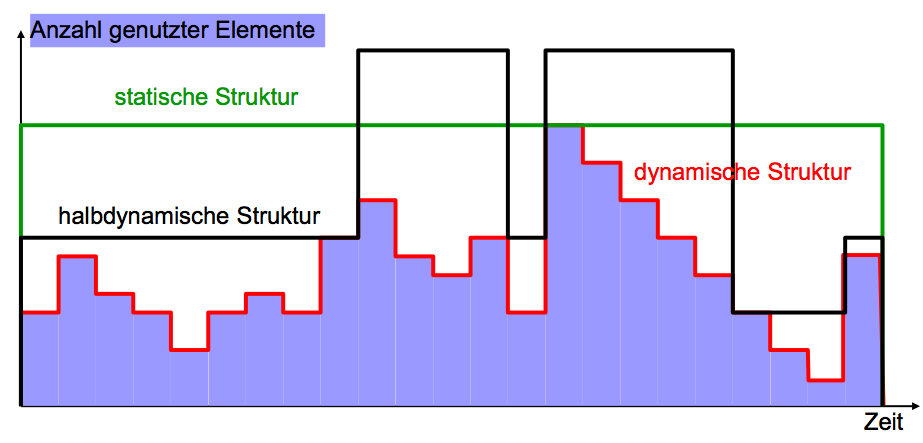
\includegraphics[width=150mm]{datennutzung_ueber_zeit.png}

\subsection{Das ArrayList}
\begin{itemize}
	\item ArrayList verwendet intern ein Array von Objekten
	\item die L\"ange des Arrays entspricht der Kapazit\"at
	\item die verwendete Anzahl Elemente ist in size gespeichert
	\item Eine ArrayList startet mit der Gr\"osse 10 wenn nicht's anderes angegeben wurde
	\item Die Kapazit\"at wird erh\"oht, wenn die ArrayList voll ist und ein neues Element hinzugef\"ugt wird.
	\item Die neue Kapazit\"at wir bei der Erh\"ohung wie folgt berechnet:\\
			JRE1.6: $cap_{new}=(cap_{old} * 3) / 2 + 1$\\
			JRE1.7: $cap_{new}=cap_{old} + (cap_{old} >> 1)$
\end{itemize}

\subsubsection{Interner Aufbau (bis Java 1.4.2)}
\begin{itemize}
	\item alle Klassen aus dem Java Collections Framework verwalten intern Referenzen vom Typ Object \\ $\Rightarrow$ maximale Flexibilit\"at
	\item alle Methodenschnittstellen verwenden den Typ Object
	\item da alle Referenztypen zur Klasse Object zuweisungskompatibel sind, bieten die Collections keine Typsicherheit
\end{itemize}

\subsubsection{Interner Aufbau (seit Java 5.0)}
\begin{itemize}
	\item alle Collections verwalten intern Referenzen vom Typ $<$E$>$, wobei E ein beliebiger Platzhalter (Typ-Parameter) f\"ur einen konkreten Referenztyp ist
	\item Collections werden generisch (maximale Flexibilit\"at)
	\item Collections k\"onnen f\"ur alle m\"oglichen Referenztypen verwendet werden, auch
f\"ur Object (= fr\"uherer interner Aufbau)
\end{itemize}

\newpage
\section{Programmverifikation}
\subsection{Korrektheit eines Algorithmus}
Ein Algorithmus heisst \Bold {korrekt}, wenn er seinen Spezifikationen gen\"ugt, wenn er zu allen Eingabedaten, die der Vorbedingung (Preconditions) gen\"ugen, die Ausgabedaten erzeugt, welche die Nachbedinungen (Postcondition) erf\"ullen. 
\begin{description}
	\item[Vorbedingung (Precondition)] \hfill \\
		Ein Algorithmus muss in einem klar definierten Zustand starten, andernfalls sind keine klaren Aussagen \"uber seine Arbeitsweise m\"oglich. Alle Parameterwerte des Algorithmus m\"ussen innerhalb der spezifizierten Wertebereiche liegen.
	\item[Nachbedingung (Postcondition)] \hfill \\
		Die Ausgabe (Endwerte) eines Algorithmus muss der Spezifikation entsprechen.
\end{description}

\subsection{Aussagelogik}
\subsubsection{Syntax}
		\begin{itemize}
			\item atomare Formeln (Atome): A, B, C, ...
			\item seien F und G zwei beliebige Formeln
				\begin{itemize}
					\item Konjunktion: $(F \wedge G)$ ist eine Formel
					\item Disjunktion: $(F \vee G)$ ist eine Formel
					\item Negation: $\neg F$ ist eine Formel
					\item Implikation: $(F \rightarrow G)$ ist eine Kurzschreibweise f\"ur $(\neg F \vee G)$
					\item Bikonditional: $(F \leftrightarrow G)$ ist eine Kurzschreibweise f\"ur $(F \ra G) \wedge (G \ra F)$
				\end{itemize}
		\end{itemize}
		
\subsubsection{Semantik}
		\begin{itemize}
				\item Belegung $\mathfrak{B}$: eine Teilmenge der atomaren Formeln wird mit einem Wahrheitswert aus {false, true} bzw. {0,1} belegt
				\item die Bedeutungen der Konjunktion, Disjunktion und Negation sind analog zur Bool'schen Algebra definiert
				\item passende Belegung $\mathfrak{B}$ auf Formel F angewendet: $\mathfrak{B}$(F)
		\end{itemize}
		
\subsubsection{Modell}
		\begin{itemize}
			\item eine Belegung heisst zu einer Formel F \Bold {passend}, wenn alle in F
vorkommenden Atome belegt sind
			\item eine Belegung $\mathfrak{B}$ ist ein \Bold {Modell} f\"ur eine Formel F, wenn sie passend ist
und wenn der Wahrheitswert von $\mathfrak{B}$(F) = true ist: $\mathfrak{B} \models F$
			\item Belegung ist $\mathfrak{B}$ \Bold {kein Modell} f\"ur Formel F, wenn sie zwar passend ist,
aber wenn der Wahrheitswert von $\mathfrak{B}$(F) = false ist: $\mathfrak{B} \nvDash F$
		\end{itemize}
		
\subsubsection{Erf\"ullbarkeit}
\begin{itemize}
	\item Eine Formel F heisst \Bold {erf\"ullbar}, wenn f\"ur sie ein Modell existiert, andernfalls \Bold {unerf\"ullbar}
	\item Eine Formel F heisst \Bold {g\"ultig} (oder Tautologie), wenn alle passenden Belegungen Modelle sind: $ \models F$
\end{itemize}

\subsubsection{\"Aquivalenz}
Zwei Formeln F und G heissen (semantisch) \"aquivalent, falls f\"ur alle passenden Belegungen $\mathfrak{B}$ gilt: $\mathfrak{B}$(F) = $\mathfrak{B}$(G). Daf\"ur schreiben wir $\models (F \leftrightarrow G)$ oder kurz $F \equiv G$. \\ \\
\begin{tabular}{l l c | c l l}
\multicolumn{2}{c}{AND} &&& \multicolumn{2}{c}{OR} \\
\hline 
&&&&& \\
$(F \wedge F)$                    & $\equiv F$                                                 &&& $(F \vee F)$ & $\equiv F$ \\
$(F \wedge G)$                   & $\equiv (G \wedge F)$                               &&& $(F \vee G)$ & $\equiv (G \vee F)$ \\
$((F \wedge G) \wedge H)$ & $\equiv (F \wedge (G \wedge H))$             &&& $((F \vee G) \vee H)$ & $\equiv (F \vee (G \vee H))$ \\
$(F \wedge (F \vee G))$      & $\equiv F$                                                 &&& $(F \vee (F \wedge G))$ & $\equiv F$ \\
$(F \wedge (G \vee H))$     & $\equiv ((F \wedge G) \vee (F \wedge H))$ &&& $(F \vee (G \wedge H))$ & $\equiv ((F \vee G) \wedge (F \vee H))$ \\
$\neg (F \wedge G)$          & $\equiv (\neg F \vee \neg G)$                    &&& $\neg (F \vee G)$ & $\equiv (\neg F \wedge \neg G)$ \\
$(F \wedge G)$                  & $\equiv G$, falls $\models F$                    &&& $(F \vee G)$ & $ \equiv G$, falls $\models F$ \\
$(F \wedge G)$                  & $\equiv$ F, falls F unerf\"ullbar                 &&& $(F \vee G)$ & $\equiv$ F, falls F unerf\"ullbar \\

\end{tabular}

\subsection{Pr\"adikatenlogik}
\subsubsection{Syntax}
\begin{itemize}
	\item Erweiterung der Aussagenlogik um Quantoren, Funktionen, Pr\"adikate, Relationen und Variablen
		\begin{itemize}
			\item nullstellige Pr\"adikate entsprechen den Atomen der Aussagelogik
			\item Relationen k\"onnen als Pr\"adikate aufgefasst werden
			\item nullstellige Funktionen sind Konstanten
		\end{itemize}
	\item Formeln
		\begin{itemize}
			\item logische Verkn\"upfung von Pr\"adikaten: \\
				die Argumente der Pr\"adikate sind Terme, gebildet aus Funktionen, Variablen und Konstanten
			\item sei x eine Variable und F eine Formel
				\begin{itemize}
					\item $\forall$ x F ist eine Formel mit gebundenem x
					\item $\exists$ x F ist eine Formel mit gebundenem x
				\end{itemize}
			\item eine Formel heisst geschlossen oder Aussage, wenn alle ihre Variablen durch Quantoren gebunden sind
		\end{itemize}
	\item Pr\"adikatenlogik mit Identit\"at \\
		wenn F und G zwei Formeln sind, so ist auch F = G eine Formel
\end{itemize}

\subsubsection{Semantik}
\begin{itemize}
	\item Struktur $S = (U_s, I_s)$ \\
		$U_s$ ist eine nicht-leere Grundmenge und IS eine Abbildung
		\begin{itemize}
			\item der Pr\"adikate \"uber $U_s$
			\item der Funktionen auf $U_s$
			\item der Variablen auf Elemente von $U_s$
		\end{itemize}
	\item Semantik bez\"uglich passender Struktur S
		\begin{itemize}
			\item[S(Term)] jeder Term wird gem\"ass $I_s$ auf ein Element aus $U_s$ abgebildet
			\item[S(Pr\"adikat)] jedes Pr\"adikat bestimmt einen Wahrheitswert in Abh\"angigkeit seiner Argumente (Terme)
			\item[S(Formel)] die aussagenlogische Verkn\"upfung der Wahrheitswerte der Pr\"adikate
			\item[S($\forall$x F)] F ist eine Formel 
				\begin{itemize}
					\item ist true, falls f\"ur alle d $\in$ US gilt: $S_{[x/d]}(F) = true$
					\item ist false, sonst
				\end{itemize}
			\item[S($\exists$x F)] F ist eine Formel
				\begin{itemize}
					\item ist true, falls f\"ur alle d $\in$ US gilt: $S_{[x/d]}(F) = true$
					\item ist false, sonst
				\end{itemize}
		\end{itemize}
\end{itemize}

\subsubsection{\"Aquivalenz}
\begin{description}
	\item[Definition] \hfill \\
		Zwei pr\"adikatenlogische Formeln F und G sind \"aquivalent, falls f\"ur alle passenden Strukturen S gilt: S(F) = S(G). Daf\"ur schreiben wir F $\equiv$ G.
	\item[\"Aquivalenzregeln (zus\"atzlich zur Aussagenlogik)] \hfill \\
		$\neg \forall x F \equiv \exists x \neg F$ \\
		$\forall x \forall y F \equiv \forall y \forall x F$ \\
		$(\forall x F \wedge \forall x G) \equiv \forall x (F \wedge G)$ \\
		$\neg \exists x F \equiv \forall x \neg F$ \\		
		$\exists x \exists y F \equiv \exists y \exists x F$ \\
		$(\exists F \vee \exists x G) \equiv \exists x (F \vee G)$ \\ \\
		falls x in G nicht frei vorkommt, gilt: \\
		$(\forall x F \wedge G) \equiv \forall x (F \wedge G)$ \\
		$(\forall x F \vee G) \equiv \forall x (F \vee G)$ \\
		$(\exists x F \wedge G) \equiv \exists x (F \wedge G)$ \\
		$(\exists x F \vee G) \equiv \exists (F \vee G)$ \\
\end{description}

\subsubsection{Beispiele}
\begin{description}
	\item[Alle Studierenden von Professor p m\"ogen Logik.] \hfill \\
		L(x) : "x mag Logik" \\
		S(x,y) : "x studiert bei y" \\
		$\forall x: S(x,p) \ra L(x)$ \\
		$\forall x: \neg S(x,p) \vee L(x)$
	\item[Ein Professor ist gl\"ucklich, wenn alle seine Studierenden Logik m\"ogen] \hfill \\
		G(x) : "x ist gl\"ucklich" \\
		$\exists y: (\forall x : S(x,y) \ra L(x)) \ra G(y)$
	\item[Ein Professor ist ungl\"ucklich, wenn er keine Studierende hat.] \hfill \\
		$\exists y: (\forall x : \neg S(x,y)) \ra \neg G(y))$
\end{description}

\subsection{Verifikation}
\subsubsection{Hoare-Tribble}
\Bold {Ein Hoare-Triple ( $\{ R \} P \{ S \}$ ) ist g\"ultig, wenn bei erf\"ullter Vorbedingung R und nach Ausf\"uhrung von P die Spezifikation (Nachbedingung) S erf\"ullt ist.} Das Programm P ist korrekt, wenn das Hoare-Triple g\"ultig ist.
\begin{description}
	\item[Variablen] \hfill \\
		Input: $a, b, c, ..., z$ \\
		Output: $a', b', c', ..., z'$
	\item[Vorbedingung (Precondition)] \hfill \\
		Damit das Programm P die Spezifikation (Postcondition) S erf\"ullen kann, muss die Vorbedingung R erf\"ullt sein. Je schw\"acher die Vorbedingung R, desto besser: \Bold {weakest precondition (WP)}.
	\item[Beispiele] \hfill \\
		Spezifikation: $S = (x' = 10)$ \\
		Programm: $P = (x' := x + 2)$ \\
		m\"ogliche Vorbedingung $R = (a = 0 \vee b = 2 \vee x = 8 \vee z = 0)$ \\
		einfachste Vorbedingung (weakest Precondition);  $WP = (x = 8)$
	\item[Nachbedingungen (Postcondition)] \hfill \\
		Die Nachbedingungen entsprechen der \Bold {Spezifikation} des Programms und sind je pr\"aziser, umso besser. \\
		Implikation: $[\underbrace{S}_{spezielle Spez.} \ra \underbrace{T}_{allg. Spez.}] \equiv \forall a, b, c, ..., z, a', b', c', ..., z': \neg S \vee T$
		\begin{itemize}
			\item $a, b, c, ..., z$ sind alle Variablen, die in den Spezifikationen S und T vorkommen
			\item wenn ein Programm P die speziellere Spezifikation S erf\"ullt, so auch die allgemeinere T
			\item es gibt ein Programm Q, welches die Spezifikation T erf\"ullt und mindestens so einfach ist wie das Programm P, welches die Spezifikation S erf\"ullt
		\end{itemize}
	\item[Besipiele:] \hfill \\
		$S = (x' = 10), T = (x' > 0)$ \\
		$P_1 = (x' := 6), P_2 = (x' := 10), P_3 = (x' := x + 1)$
		\begin{itemize}
			\item $\underbrace{\{true\}}_{algemeinste Vorbedingung} P_1 \{S\} = false$
			\item $\{true\} P_1 \{T\} = true$
			\item $\{true\} P_2 \{S\} = true$
			\item $\{true\} P_2 \{T\} = true$
			\item $\{true\} P_3 \{S\} = false$
			\item $\{x=9\} P_3 \{S\} = true$
		\end{itemize}
\end{description}

\subsubsection{Ablauf der Verifikation}
\begin{description}
	\item[Gegeben] \hfill \\ \\
		Vorbedingung R, Spezifikation S, Programm P
	\item[Ablauf] \hfill 
		\begin{itemize}
			\item aus S und P die schw\"achste Vorbedingung $WP = wp(P, S)$ berechnen
			\item falls $[R \ra WP]$ gilt, dann erf\"ullt das Programm P die Spezifikation S bei eingehaltener Vorbedingung R
			\item R kann somit durch WP ersetzt werden
		\end{itemize}
	\item[Berechnung der WP] \hfill 
		\begin{itemize}
			\item ausgehend von der Spezifikation S
			\item Anweisung f\"ur Anweisung r\"uckw\"arts rechnen
			\item Berechnungsregeln f\"ur Zuweisung, Sequenz, Selektion, Iteration
		\end{itemize}
\end{description}

\subsection{Weakest Precondition: Rechenregeln}
\subsubsection{Zuweisung}
\begin{description}
	\item[Gegeben] \hfill \\
		Zuweisung $P = (x' := y)$ \\
		Nachbedingung S
	\item[Regel] \hfill \\
		$WP = wp(P, S) = wp((x' := y), S) = S |_{alle \hspace{2mm} x' \hspace{2mm} durch \hspace{2mm} y \hspace{2mm} ersetzt}$
	\item[Beispiele] \hfill \\
		$S = (a' = z), P = (a' := b + c), WP = (b + c = z)$ \\
		$S = (n' = n), P = (n' := n-1), WP = (n = n-1) = false$
\end{description}

\subsubsection{Sequenz}
\begin{description}
	\item[Gegeben] \hfill \\
		Sequenz P = $(Anweisung_1; Anweisung_2; ...; Anweisung_n)$ \\
		Nachbedingung S
	\item[Regel] \hfill \\
		$WP = wp(P, S) =
wp((Anweisung_1; Anweisung_2; ...; Anweisung_{n-1}), wp(Anweisung_n, S))$
	\item[Beispiel] \hfill \\
		$P = (t' := x; x' := y; y' := t')$ \\
		$S = (x' = b \wedge y' = a)$ \\
		$WP =wp((t':=x;x':=y;y':=t'),(x'=b \wedge y'=a))$ \\
		$= wp((t' := x; x' := y), wp((y' := t'), (x' = b \wedge y' = a)))$ \\
		$= wp((t' := x; x' := y), (x' = b \wedge t' = a))$ \\
		$= wp((t' := x), wp((x' := y), (x' = b \wedge t' = a)))$ \\
		$= wp((t' := x), (y = b \wedge t' = a))$ \\
		$= (y = b \wedge x = a)$
\end{description}

\subsubsection{Selektion}
\begin{description}
	\item[Gegeben] \hfill \\
		logischer Ausdruck b \\
		Selektion P= (if b then $P_1$ else $P_2$) \\
		Nachbedingung S
	\item[Regel] \hfill \\
		$WP = wp(P, S) = wp(($ if b then $P_1$ else $P_2), S)$ \\
		$=\textcolor{red}{(\neg b \vee wp(P_1,S)) \wedge (b \vee wp(P_2,S))}$ \\
		$=\textcolor{blue}{b \wedge wp(P_1,S)\vee \neg b \wedge wp(P_2,S)}$
	\item[Beispiel] \hfill \\
		$P = (if x < 0 then x' := -x else x' := x – 1)$ \\
		$S = (x' > 0)$ \\
		$WP = wp((if x < 0 x' := -x else x' := x – 1), x' > 0)$ \\
		$=\textcolor{red}{(x \geq 0 \vee -x > 0) \wedge (x < 0 \vee x – 1 > 0)}$ \\
		$= (x ≥ 0 \vee x < 0) \wedge (x < 0 \vee x > 1)$ \\
		$= true \wedge (x \notin [0, 1])$ \\
		$= x \notin [0, 1]$ \\
		$=\textcolor{blue}{(x < 0 \wedge -x > 0) \vee (x ≥ 0 \wedge x - 1 > 0)}$ \\
		$= (x < 0) \vee (x ≥ 0 \wedge x > 1)$ \\
		$= (x < 0) \vee (x > 1)$ \\
		$= x \notin [0, 1]$
\end{description}

\subsubsection{Iteration}
\begin{description}
	\item[Iterationen] \hfill \\
		for-Schleife: Anzahl Durchl\"aufe bekannt $\ra$ als Sequenz betrachten \\
		while-Schleife: Spezialfall der Rekursion $\ra$ Invariante bestimmen
	\item[Invariante (INV)] \hfill \\
		eine logische Bedingung ausgedr\"uckt in den Variabeln aus P, welche vor P und nach jedem durchlauf von $P_1$ g\"ultig ist \\
		wenn $\{INV \wedge B\} P_1 \{ INV \}$ g\"ultig ist, so ist auch  $\{INV \}$ while B do $P_1 \{ INV \wedge \neg B \}$ g\"ultig
	\item[Regel] \hfill \\
		WP = wp(P,S) = INV
\end{description}

\subsection{Invarianten-Anwendung}
\begin{lstlisting}
long multiply(int x, int y) {
	\Bold {// 4. schwaechste Vorbedingung WP}
	long a = x, b = y, r = 0;
	// 3. INV muss gelten
	while (a != 0) {
		// 2. INV & (a!=0) muss gelten
		if ((a & 1) == 1) r += b;
		b = b << 1;
		a = a >> 1;
		// 1. INV muss gelten
	} // 5. INV & (a = 0) muss gelten
	return r;
} //Nachbedingung S muss gelten
\end{lstlisting}
\subsubsection{Ist INV wirklich eine korrekte Invariante?}
\begin{description}
	\item[Gegeben] \hfill \\
		Invariante INV $= (a \geq 0 \wedge a*b + r = x*y)$ 
	\item[Beweisverfahren] \hfill \\
		wenn an Position 1 die Invariante INV gilt, dann muss an der Position 2 auch die Invariante gelten \\
		zu zeigen: $\{ (INV \wedge B) \ra wp(P1, INV) \}$
	\item[Beispiel] \hfill \\
		R1 = wp(a := a $>>$ 1, INV) $= (\frac{a}{2} \geq 0 \wedge \frac{a}{2}*b + r = x*y)$ \\
		R2 = wp(b := b $<<$ 1, R1) $= (\frac{a}{2} \geq 0 \wedge \frac{a}{2}*b*2 + r = x*y)$ \\
		R3 = wp((if (a\&1) = 1 then r := r + b else NOP), R2) $= \frac{a}{2} \geq 0 \wedge a*b + r = x*y$
\end{description}

\subsubsection{Was ist die schw\"achste Vorbedingung WP?}
\begin{description}
	\item[Gegeben] \hfill \\
		Invariante INV $= (a \geq 0 \wedge a*b + r = x*y)$ 
	\item[Beweisverfahren] \hfill \\
		Wenn an Position 2 die Invariante INV gilt, dann gilt sie auch an der Position 3. \\
		Somit ist INV an der Position 3 die Nachbedingung der Instruktionen vor der while-Schleife und wir k\"onnen mit dem \"ublichen Verfahren WP berechnen.
	\item[Beispiel] \hfill \\
		R1 = wp(r := 0, INV) $= (a \geq 0 \wedge a*b = x*y)$ \\
		R2 = wp(b := y, R1) $= (a \geq 0 \wedge a*y = x*y)$ \\
		WP = wp(a := x, R3) $= (x \geq 0 \wedge x*y = x*y) = (x \geq 0)$
\end{description}

\subsubsection{Welches ist die Nachbedingung S?}
\begin{description}
	\item[Gegeben] \hfill \\
		Invariante INV $= (a \geq 0 \wedge a*b + r = x*y)$ \\
		Schleifenbedingung B $= (a \neq 0)$
	\item[Verfahren] \hfill \\
		Wenn an Position 1die Invariante INV gilt, dann gilt an der Position 5 die Invariante, nicht aber B, also S $= (INV \wedge \neg B)$
	\item[Beispiel] \hfill \\
		$S = (INV \wedge \neg B) = (a \geq 0 \wedge a*b + r = x*y \wedge a = 0)$ \\
		$S = (r = x*y \wedge a = 0)$ \\
		Der R\"uckgabewert r ist also gleich dem Produkt aus x und y.
\end{description}

\newpage
\section{Komplexit\"at}

\subsection{Zeit- und Speicherbedarf}
\begin{description}
	\item[Modell: Random-Access-Machine (RAM)] \hfill \\
		Eine m\"oglichst einfache CPU mit einem unendlich grossen Speicher bestehend aus Zellen f\"ur beliebig grosse Zahlen.
		\item[Speicherbedarf eines Algorithmus] \hfill \\
			Die minimale Anzahl Speicherzellen im RAM-Modell, die vorhanden sein m\"ussen, damit der Algorithmus korrekt ausgef\"uhrt werden kann.
		\item[Zeitbedarf eines Algorithmus] \hfill \\
			\Bold {Laufzeit in Echtzeit}: gemessene Ausf\"uhrungszeit eines Programms mit vordefinierten Testdaten auf einem pr\"azise beschriebenen Computersystem. \\
			\Bold {Laufzeit in RAM-Instruktionen}: die minimale Anzahl RAM-Befehle, die ausgef\"uhrt werden m\"ussen, um den Algorithmus abzuarbeiten.
		\item[Definitionen] \hfill \\
			Laufzeit: T(n) \\
			Speicherbedarf: M(n)
\end{description}

\subsection{Worst-Case vs. Average-Case}
\begin{description}
		\item[Best-Case (meistens uninteressant)] \hfill \\
			die Zahlen sind bereits sortiert
		\item[Worst-Case (sinnvoll und praktikabel)] \hfill \\
			die Zahlen sind in umgekehrter Reihenfolge
		\item[Average-Case (oft zu schwierig)] \hfill \\
			Um eine Aussage der Art \"{ }Im Durchschnitt dauert es\"{ }  machen zu k\"onnen, muss Klarheit bestehen, wor\"uber der Durchschnitt gebildet werden darf. Fairerweise m\"ussen alle m\"oglichen Probleminstanzen der L\"ange n mit ihrer Wahrscheinlichkeitsverteilung in Betracht gezogen werden.
\end{description}

\subsection{Gross-O und Gross-Omega}
\subsubsection{Gross-O}
\begin{itemize}
	\item obere Schranke einer Worst-Case Absch\"atzung
	\item sinnvoll f\"ur konkrete Algorithmen
	\item Beispiel: \\
		n Zahlen k\"onnen mit Heap-Sort in Zeit T(n) $\in \mathcal{O}$(n log n) bei einem
Speicherbedarf M(n) $\in \mathcal{O}$(n) sortiert werden
\end{itemize}
\subsubsection{Gross-Omega}
\begin{itemize}
	\item untere Schranke einer Worst-Case Absch\"atzung
	\item sinnvoll f\"ur Problemklassen
	\item Beispiel: \\
		um n beliebige Zahlen in beliebiger Reihenfolge auf einer RAM zu sortieren, braucht es mindestens $\Omega$(n log n) Rechenschritte \\
	\Bold {Formal}: $ \Omega (g(n))  = \{  h(n) | \exists c > 0 : \exists $ unendlich viele $n:h(n) \geq c * g(n) \}$
	\item Gross-Theta: Sind $\mathcal{O}$ und $\Omega$ gleich wird  geschrieben: $T(f) \in \Theta(g)$ \\
	Kann gelesen werden als: \glqq $f$ w\"achst genauso schnell wie $g$\grqq
\end{itemize}

\newpage
\section{Rekursion}



\subsubsection{Formeln}

Der kleine Gauss:\\
$\sum_{k=0}^n{k} = 0+1+2+...+n = \frac{n(n+1)}{2}$ 
\\\\
Beispiele:\\
$\sum_{k=0}^{n-1}{k} =  \frac{(n-1)(n-1+1)}{2} = \frac{n(n-1)}{2}$
\\\\
$\sum_{k=0}^{n-1}{n-k} = \sum_{k=1}^{n}{n} - \sum_{k=0}^{n-1}{k} =
n^2 - \frac{n(n-1)}{2}$\\


\newpage
\section{Divide-and-Conquer}
\begin{itemize}

	\item[Divide 1.)]
		Gesamtproblem in 2 oder 3 gleichgrosse Teilprobleme zerlegen
	\item[Conquer 2.)] 
		jedes Teilproblem separat l\"osen (gleicher Algorithmus wie f\"urs Gesamtproblem)
	\item[Merge 3.)] 
		aus Teill\"osungen die Gesamtl\"osung erzeugen.
\end{itemize}

\subsection{Code-Listing}
\begin{lstlisting}
int maxTSumme(int[] a, int left, int right) {
	if (left > right) return 0;
	if (left == right) return (a[left] >= 0 ? A[left] : 0);
	int m = (left + right) >>> 1;
	int v1 = maxTSumme(a, left, m)
	int v2 = maxTSumme(a, m+1, right);
	int sum=0; rmax=0; lmax=0;
	for (int i=m+1; i <= right; i++) {
		sum += a[i];
		if (sum > rmax) rmax =  sum;
	}
	sum = 0;
	for (int i=m; i>=left; i--) {
		sum += a[i];
		if (sum > lmax) lmax = sum;
	}
	int v3 = lmax + rmax;
	return max(v1, v2, v3);
}
\end{lstlisting}
\subsection{Analyse}
\subsubsection{Schritte}
\begin{itemize}
	\item[Zeile 2-4:] 10 Schritte
	\item[Zeile 5:] $T(\frac{n}{2})$ Schritte
	\item[Zeile 6:] $T(\frac{n}{2})$ Schritte
	\item[Zeile 8 - 16:] $6 + 6*n$ Schritte
	\item[Zeile 17 - 18:] 5 Schritte
\end{itemize}
n: l\"ange von a
\subsubsection{Aufwandsformel}
$T(n) = 2* T(\frac{n}{2	}) + 6n + 21$ \\
$T(1) = 7$

\subsection{Berechnung}
\subsubsection{Teleskopieren}
$T(n) = 2 * \underline{T(\frac{n}{2})} + 6*n +21$ \\
$T(n) = 2 * (\underline{2*T(\frac{n}{4}) + \frac{6*n}{2} +21 } ) + 6*n + 21$ \\
$T(n) = 4 * \underline{T(\frac{n}{4})} + 12 * n + 3* 21$ \\
$T(n) = 4 * (\underline{2*T(\frac{n}{8}) + \frac{6*n}{4} +21 } ) + 12*n + 3*21$ \\
$T(n) = 8 * \underline{T(\frac{n}{8})} + 18 * n + 7* 21$ 
\subsubsection{Verallgemeinerung}
$T(n) = 2^i*T(\frac{n}{2^i}) +6*i*n +(2^i-1)*21$ \\  \\
$\frac{n}{1^i} = 1 \Ra n=2^i \Ra i = log_2(n) =  ld(n)$ \\ \\
$T(n) = 2^{ld(n)} * T(1) +6*ld(n)*n + (2^{ld(n)} -1) * 21$ \\
$T(n) = n*7 + 6*ld(n)*n +(n-1)*21$ \\
$T(n) = 6*n*ld(n)+28*n-21$
\end{document}
